\documentclass[class=jsarticle, crop=false, dvipdfmx, fleqn]{standalone}
\input{/Users/User/Documents/TeX/preamble/mypreamble}
\begin{document}
\section*{練習問題5-1}
中古車価格データの全てをプロットすると,
以下の図\ref{fig:q_5_1_all_data}のようになる。

\begin{figure}[H]
\centering
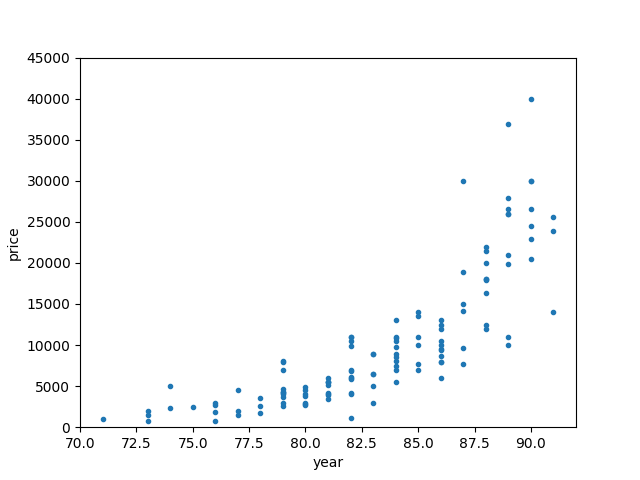
\includegraphics[clip, width=12cm]{../figures/q_5_1_all}
\caption{【練習問題5-1】 中古車価格データの完全版}
\label{fig:q_5_1_all_data}
\end{figure}

これについて1~4次式モデルで多項式回帰を行う。
ここでは最小二乗法を用いて解を求めることとする。

モデルの優劣の決め方について述べる。
まず完全版データを教師データとテストデータに分け,
教師データを用いてモデルを求め,
テストデータでそのモデルを評価する。
教師データは乱数によって選択することとし,
その乱数のseedをいくつか変えて複数回試行を行う。
モデル作成時のAICcとテストデータに対する$Q$(最小二乗和)を求め,
それらを単純平均することによってモデルの評価を行う。

なお,赤池情報量基準については,
$n$が小さいことから,
\begin{equation}
\mathrm{AICc} = n \log{\frac{\hat{Q}}{n}} + \frac{2kn}{n - k - 1}
\end{equation}
を用いる。

ここでは試行回数を100回とする。
また,配布資料に倣って,教師データの数を10としてモデルを求めたところ,
その結果は以下のようになった。
なお,図は適当なseedのときのモデルをプロットしたものである。

\begin{table}[H]
\centering
\caption{【練習問題5-1】 テストデータ10個のときの各次元に対するAICcと$Q$の平均値}
\begin{tabular}{|ccc|} \hline
次元 & AICc & $Q$ \\ \hline
1 & 205.27 & \num{3.80851e9} \\
2 & 215.66 & \num{3.80475e9} \\
3 & 282.89 & \num{4.98813e10} \\
4 & 116.06 & \num{3.60880e10} \\ \hline
\end{tabular}
\label{tab:q_5_1_result_10}
\end{table}

%\begin{figure}[H]
%\centering
\begin{figure}[H]%{0.45\linewidth}
	\centering
	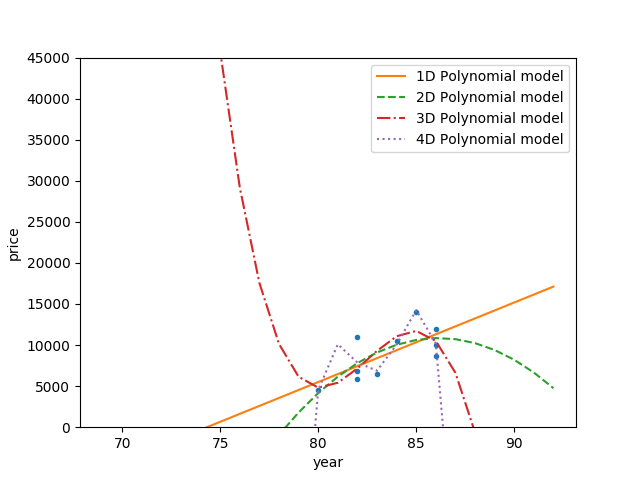
\includegraphics[clip, width=0.8\linewidth]{../figures/q_5_1_train_10}
	\caption{テストデータ10個のときのtrain時のfittingの図}
	\label{fig:q_5_1_train_10}
\end{figure}
\begin{figure}[H]%{0.45\linewidth}
	\centering
	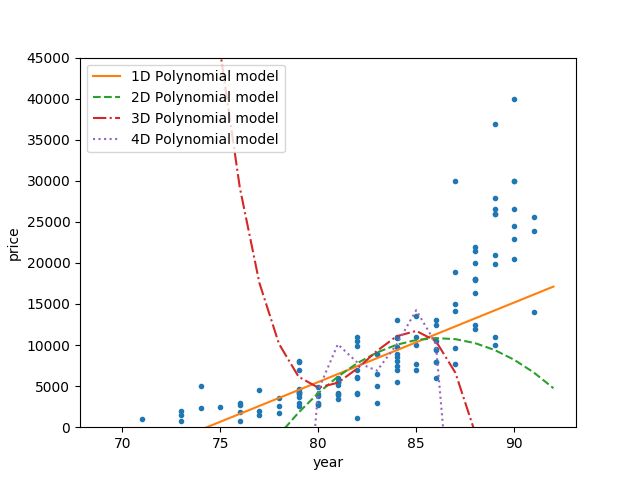
\includegraphics[clip, width=0.8\linewidth]{../figures/q_5_1_test_10}
	\caption{テストデータ10個のときのtest時のfittingの図}
	\label{fig:q_5_1_test_10}
\end{figure}
%\end{figure}

表\ref{tab:q_5_1_result_10}より,
AICcの値からすれば4次が,
$Q$の値からすれば1,2次が優れているといえるが,
図\ref{fig:q_5_1_train_10},\ref{fig:q_5_1_test_10}を見れば2,4次は妥当ではないと思われる。
これは,テストデータが少なすぎるため,
2次ではうまくfitできず,
また4次では過学習してしまってAICcが小さくなっているのだと考えられる。
従って1次式が優れたモデルである,と言えなくもないが,
元データは1次式というよりは曲線に見える。

以上の問題はテストデータが少なすぎたために起こっていると考えられる。
そこで,全てのデータの30{\%}をテストに利用した場合について調べてみたところ,
その結果は以下のようになった。

\begin{table}[H]
\centering
\caption{【練習問題5-1】 テストデータ30{\%}のときの各次元に対するAICcと$Q$の平均値}
\begin{tabular}{|ccc|} \hline
次元 & AICc & $Q$ \\ \hline
1 & 671.43 & \num{2.51412e9} \\
2 & 662.66 & \num{1.84339e9} \\
3 & 667.49 & \num{1.94358e9} \\
4 & 676.40 & \num{2.32340e9} \\ \hline
\end{tabular}
\label{tab:q_5_1_result_30per}
\end{table}

%\begin{figure}[H]
%\centering
\begin{figure}[H]%{0.45\linewidth}
	\centering
	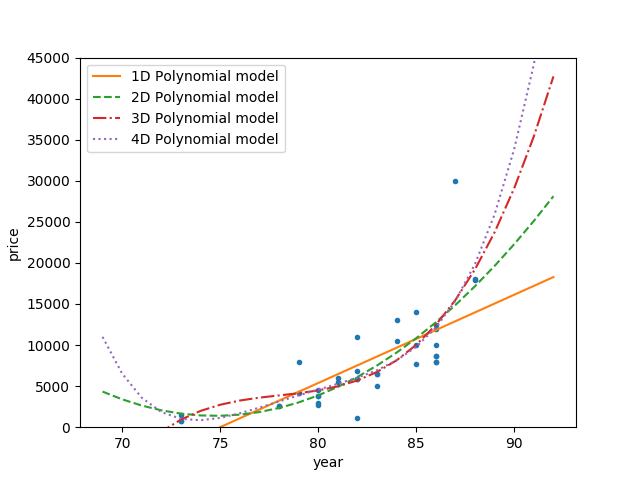
\includegraphics[clip, width=0.8\linewidth]{../figures/q_5_1_train_30per}
	\caption{テストデータ30{\%}のときのtrain時のfittingの図}
	\label{fig:q_5_1_train_30per}
\end{figure}
\begin{figure}[H]%{0.45\linewidth}
	\centering
	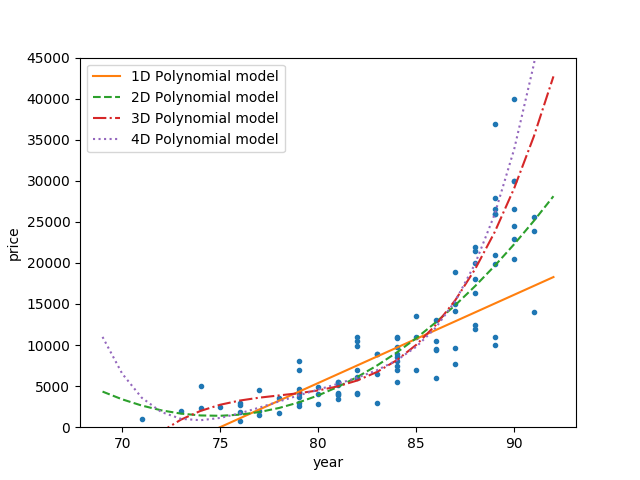
\includegraphics[clip, width=0.8\linewidth]{../figures/q_5_1_test_30per}
	\caption{テストデータ30{\%}のときのtest時のfittingの図}
	\label{fig:q_5_1_test_30per}
\end{figure}
%\end{figure}

表\ref{tab:q_5_1_result_30per}より,
テストデータを全体の30{\%}としたところ,
AICc,$Q$ともに2次が最も優れている。
また,図を見ても大きな違和感はない。

以上の考察により,
2次式モデルが最も優れているといえる。


\end{document}